\newpage
\section{模型的建立与求解}

\subsection{统一的固定域热湿输运模型}

\subsubsection{建模思路与局部守恒}

四问虽然在物性、时间范围和几何上逐步增加复杂性，但热量和水分都遵循同一条“控制体内积累量等于净流入量”的主线。为避免把干基含水率误作体积浓度，先在半径$r$处取厚度为$\mathrm dr$的同心薄环。记径向向外为正方向，导热通量和相对干固体的水分通量分别为
\begin{equation}
q_T=-k(C)\frac{\partial T}{\partial r},\qquad
q_C=-D(C,T)\frac{\partial C}{\partial r}.
\label{eq:constitutive-flux}
\end{equation}
薄环的外、内表面积分别为$2\pi(r+\mathrm dr)L$和$2\pi rL$。将净流入量除以薄环体积并令$\mathrm dr\to0$，可得
\begin{equation}
b(C)\frac{\partial T}{\partial t}
=-\frac{1}{r}\frac{\partial(rq_T)}{\partial r},\qquad
\frac{\partial C}{\partial t}
=-\frac{1}{r}\frac{\partial(rq_C)}{\partial r}.
\label{eq:local-balance}
\end{equation}
这里$b(C)=\hat\rho(C)c_p(C)$作为题给经验关系下的有效体积热容，水分方程则按单位干固体质量归一化。两式的守恒测度不同，正是后续不能直接把$\hat\rho C$写入水分积累项的原因。

\subsubsection{控制方程}

记圆柱初始半径为$R_0=0.02$ m，长度为$L=0.25$ m。对固定几何问题，在忽略轴向变化后，圆柱径向热传导与干基水分扩散方程写为
\begin{equation}
 b(C)\frac{\partial T}{\partial t}
 =\frac{1}{r}\frac{\partial}{\partial r}
 \left(rk(C)\frac{\partial T}{\partial r}\right),
 \label{eq:heat-fixed}
\end{equation}
\begin{equation}
 \frac{\partial C}{\partial t}
 =\frac{1}{r}\frac{\partial}{\partial r}
 \left(rD(C,T)\frac{\partial C}{\partial r}\right).
 \label{eq:moist-fixed}
\end{equation}
式\eqref{eq:heat-fixed}、\eqref{eq:moist-fixed}由式\eqref{eq:constitutive-flux}代入式\eqref{eq:local-balance}得到。式\eqref{eq:moist-fixed}中的$C$是单位干药材质量所含水分，不是单位体积水浓度；固定域中干固体密度在归一化方程两侧约去。热方程写成$b(C)T_t$而非$[b(C)T]_t$，对应本文采用的有效显热闭合；变系数引起的收支修正将在模型检验中单独核验。

初始条件为
\begin{equation}
 T(r,0)=28\ ^\circ\mathrm C,\qquad C(r,0)=2.55.
 \label{eq:initial}
\end{equation}
中心满足对称条件，侧表面满足Robin边界：
\begin{equation}
 \left.\frac{\partial T}{\partial r}\right|_{r=0}=0,
 \quad
 \left.\frac{\partial C}{\partial r}\right|_{r=0}=0,
 \label{eq:center-bc}
\end{equation}
\begin{equation}
 -k\left.\frac{\partial T}{\partial r}\right|_{r=R_0}
 =h(T_s-T_{\mathrm{air}}),
 \quad
 -D\left.\frac{\partial C}{\partial r}\right|_{r=R_0}
 =h_m(C_s-C_{\mathrm{eq}}).
 \label{eq:surface-bc}
\end{equation}
加热阶段$T_s<T_{\mathrm{air}}$，故式\eqref{eq:surface-bc}的热通量为负，表示热量沿径向向内传递；排湿阶段$C_s>C_{\mathrm{eq}}$，水分向外通量为正，符号与物理方向一致。

\subsubsection{真实表面值与边界闭合}

题目要求给出$r=R$处结果，而有限体积未知量位于最外层控制体中心$r_N<R$。若直接用$T_N,C_N$代替表面值，会在Robin边界处引入半个网格宽度的系统偏差。记$\delta_s=R-r_N$，将最后半单元扩散阻力与外部膜阻力串联，有
\begin{equation}
\frac{T_N-T_s}{\delta_s/k_{N,s}}=h(T_s-T_{\mathrm{air}}),
\label{eq:surface-heat-closure}
\end{equation}
\begin{equation}
\frac{1}{\delta_s}\int_{C_s}^{C_N}D(C,\bar T_{N,s})\,\mathrm dC
=h_m(C_s-C_{\mathrm{eq}}).
\label{eq:surface-moist-closure}
\end{equation}
常物性时式\eqref{eq:surface-heat-closure}就是两段热阻的显式串联；变物性时，$k$在半单元平均含水率处更新，式\eqref{eq:surface-moist-closure}保留$D$对$C$的变化，并与表面温度联立求解。程序使用区间保护的牛顿迭代，必要时退化为有界标量求根，因此得到的是满足边界方程的真实表面值，而非外推值。

\subsubsection{环形有限体积离散}

将径向区域划分为表面加密的$N=1280$个环形控制体，边界节点取
\begin{equation}
 r_j=R_0\left[1-\left(1-\frac{j}{N}\right)^2\right],\qquad j=0,1,\ldots,N.
\end{equation}
第$i$个控制体体积和内外侧面积分别为
\[
V_i=\pi L(r_{i+1/2}^2-r_{i-1/2}^2),\qquad
A_{i\pm1/2}=2\pi Lr_{i\pm1/2}.
\]
对任意场$\phi\in\{T,C\}$，令$\Gamma=k$或$D$，内部面向外通量采用两侧半网格阻力串联：
\begin{equation}
q_{i+1/2}=
\frac{\phi_i-\phi_{i+1}}
{(r_{i+1/2}-r_i)/\Gamma_i+(r_{i+1}-r_{i+1/2})/\Gamma_{i+1}}.
\label{eq:harmonic-flux}
\end{equation}
于是半离散方程统一写成
\begin{equation}
M_i\frac{\mathrm d\phi_i}{\mathrm dt}
=A_{i-1/2}q_{i-1/2}-A_{i+1/2}q_{i+1/2},
\quad
M_i=\begin{cases}b_iV_i,&\phi=T,\\V_i,&\phi=C.\end{cases}
\label{eq:fvm-semidiscrete}
\end{equation}
中心面取$q_{1/2}=0$，外表面通量由式\eqref{eq:surface-bc}给出。相邻控制体在公共面使用完全相同、符号相反的通量，求和后所有内部通量逐项抵消，因而离散层面保持局部与整体守恒。表面加密网格则把计算资源集中到温湿梯度最大的区域。

\subsubsection{时间积分与结果重建}

离散后得到$2N$维非线性刚性常微分方程组。本文采用带解析稀疏Jacobian的变步长BDF方法\cite{virtanen2020}，并按以下步骤求解：
\begin{enumerate}[label=\arabic*)]
  \item 读取附件观测并构造分段线性环境函数；在每个观测折点前后分别积分，避免求解器跨越导数不连续点；
  \item 在每次右端函数计算中，由当前$T_i,C_i$更新$b,k,D$，计算内部面通量和真实表面状态；
  \item BDF根据局部误差自适应选取内部步长，题定的1 s或60 s只作为稠密输出间隔；
  \item 用中心偶对称二次式、内部区间保形三次插值和边界闭合值重建题定半径处结果；
  \item 对问题三、四继续在每个积分片段内搜索全域事件，并在事件后独立推进以核验严格不等式。
\end{enumerate}

主计算设置见表\ref{tab:numerical-settings}。统一采用$N=1280$和二次表面加密；相对容差取$10^{-10}$，温度与含水率绝对容差分别为$10^{-11}$和$10^{-13}$。指定径向位置的场值采用保形分段三次重建，避免普通高阶插值在陡峭表面层产生过冲\cite{fritsch1980}。

\begin{table}[htbp]
  \caption{主计算设置}
  \label{tab:numerical-settings}
  \centering
  \begin{tabular}{clccc}
    \toprule
    问题 & 积分区间 & 最大内部步长/s & 输出间隔/s & 初态来源 \\
    \midrule
    一 & $0$--$1800$ s & 1 & 1 & 原始均匀初态 \\
    二 & $0$--$3$ h & 2 & 1 & 原始均匀初态 \\
    三 & $3$ h--阈值事件 & 30 & 60 & 问题二全精度末态 \\
    四 & $0$--阈值事件 & 30 & 60 & 原始均匀初态 \\
    \bottomrule
  \end{tabular}
\end{table}

\subsection{问题一：解耦预热模型}

\subsubsection{物性与模型特点}

问题一采用附录二常热物性
\[
\hat\rho=820,\qquad c_p=2600,\qquad k=0.36,
\]
以及含水率相关扩散率
\begin{equation}
D(C)=7\times10^{-9}\exp\left(-\frac{0.89}{C}\right)\ \mathrm{m^2/s}.
\label{eq:q1-D}
\end{equation}
由于热方程系数不依赖$C$，且式\eqref{eq:q1-D}不依赖$T$，两场在本问中相互解耦。它们仍共享同一时变环境时间轴，但可分别积分。

\subsubsection{求解过程与尺度判断}

将常热物性代入式\eqref{eq:heat-fixed}，热扩散率为
\begin{equation}
\alpha=\frac{k}{\hat\rho c_p}=1.6886\times10^{-7}\ \mathrm{m^2/s}.
\end{equation}
初态下$D(C_0)=4.9376\times10^{-9}\ \mathrm{m^2/s}$。在$t=1800$ s时，以$\ell\sim\sqrt{at}$估计，热扩散长度和水分扩散长度分别约为$1.743$ cm和$0.298$ cm。前者已接近半径$2$ cm，后者仅覆盖外层约$15\%$的径向距离，预示温度剖面会整体抬升，而含水率会形成明显表面层。

具体计算时分别构造$N$维热方程和水分方程。热问题的系数矩阵只随网格和常物性确定；水分问题则在每个BDF内部步重新计算$D(C_i)$。由于
\begin{equation}
\frac{\mathrm dD}{\mathrm dC}=D(C)\frac{0.89}{C^2}>0,
\end{equation}
表层失水会使当地扩散率下降，产生一定的自抑制作用。两场求解完成后再在统一的1 s时间轴和0.1 cm径向网格上重建输出，保证温湿结果能够逐点对应。

\subsubsection{结果与分析}

题定温度和含水率结果分别见表\ref{tab:q1_temperature}、表\ref{tab:q1_moisture}。

\input{tables/q1_tables}

图\ref{fig:q1-fields}给出完整时空演化。30 min时，中心、表面温度分别达到$33.5753\ ^\circ\mathrm C$和$36.7856\ ^\circ\mathrm C$，横截面加权平均温度为$35.1679\ ^\circ\mathrm C$；同期中心含水率仍为$2.5500$，表面已降至$1.5102$，加权平均为$2.2936$。初态估计的热扩散长度约$1.743$ cm，水分扩散长度仅约$0.298$ cm，与“热影响进入内部而显著失水集中于表层”的计算结果一致。

\begin{figure}[htbp]
  \centering
  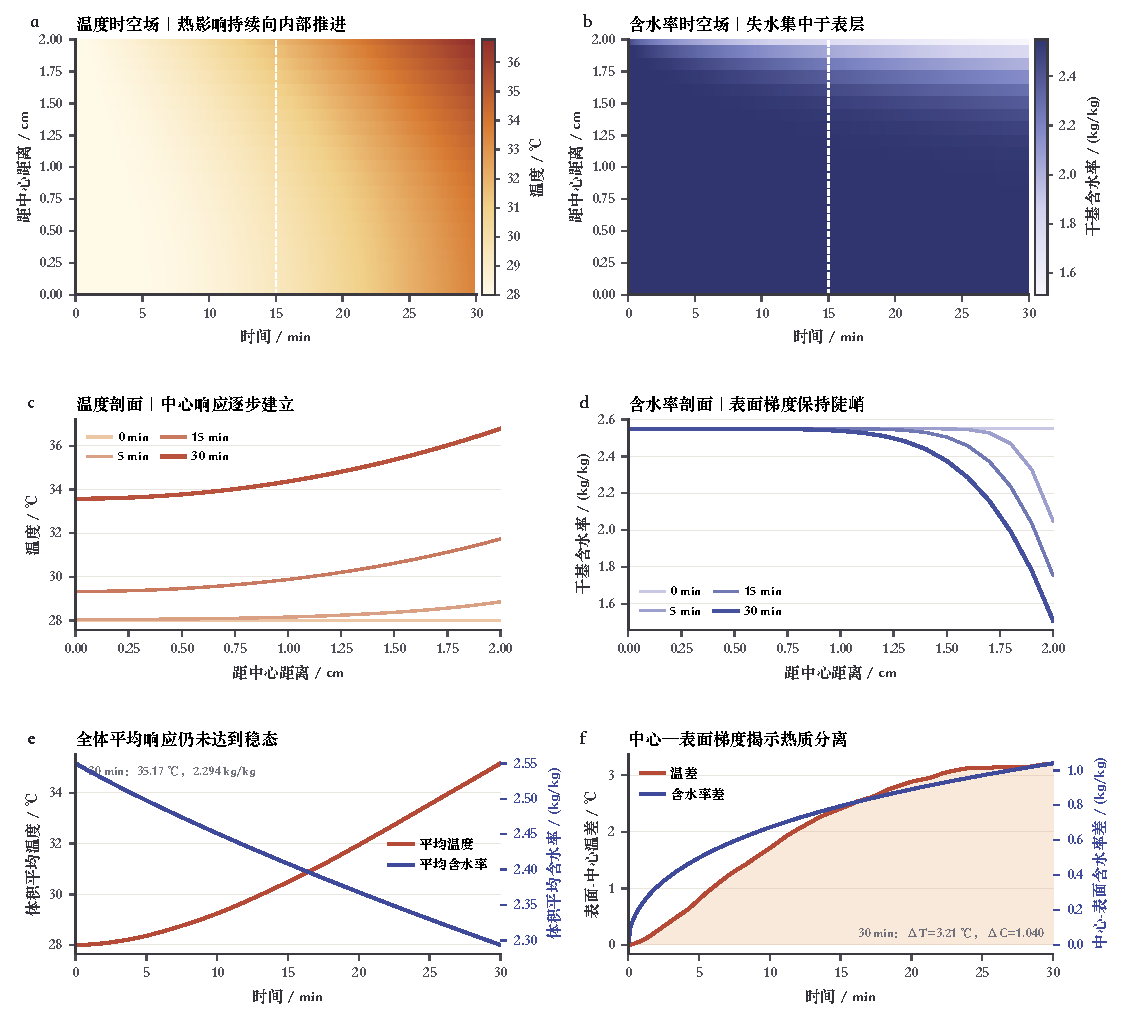
\includegraphics[width=\textwidth]{figures/fig02_q1_fields.pdf}
  \caption{问题一温湿场演化}
  \label{fig:q1-fields}
\end{figure}

图\ref{fig:q1-fields}(a)(b)从时空场展示传播范围，(c)(d)用同一组时刻的径向剖面揭示梯度形状，(e)(f)再把局部场压缩为体积平均响应和中心---表面差。30 min时温差与含水率差分别达到$3.2103\ ^\circ\mathrm C$和$1.0398$，二者仍同步增大；因此表面含水率快速下降并不意味着出现锐利的干燥前沿。中心值在四位小数下暂未变化，也不等于中心水分在数学上绝对静止，而是早期变化小于显示分辨率。

从加权平均量看，30 min时温度已由$28\ ^\circ\mathrm C$升至$35.1679\ ^\circ\mathrm C$，完成了相对于同期环境温度的大部分响应；平均含水率仍为$2.2936$，保留初始值的约$89.9\%$。这组对比从整体量和局部剖面两方面验证了尺度分析，不依赖某一个抽样半径的偶然结果。

\subsection{问题二：变物性热湿耦合模型}

\subsubsection{耦合关系}

问题二使用附录三物性：
\begin{align}
\hat\rho(C)&=650+128C,\\
c_p(C)&=1450+2736\frac{C}{1+C},\\
k(C)&=0.21+0.38\frac{C}{1+C},
\end{align}
\begin{equation}
D(C,T)=2.4\times10^{-3}
\exp\left(-\frac{0.45}{C}\right)
\exp\left[-\frac{3850}{T+273.15}\right].
\label{eq:q23-D}
\end{equation}
温度升高使式\eqref{eq:q23-D}增大，含水率降低则使其减小；与此同时，$C$还通过$b(C)$和$k(C)$改变温度响应，由此形成物性系数介导的双向反馈。数值求解时在每次残差计算中更新全部局部系数，并保留散度算子内部的变系数$\nabla\cdot(k\nabla T)$。

由扩散率经验式直接求偏导，有
\begin{equation}
\frac{\partial\ln D}{\partial T}
=\frac{3850}{(T+273.15)^2}>0,
\qquad
\frac{\partial\ln D}{\partial C}=\frac{0.45}{C^2}>0.
\label{eq:D-partials}
\end{equation}
因此升温促进内部扩散，而失水通过降低$C$抑制扩散。另一方面，$\hat\rho(C)$、$c_p(C)$和$k(C)$均随$C$增加；脱水会同时减小体积热容和导热系数，前者倾向于加快局部升温，后者倾向于增强温度梯度。两类作用方向不同，需要联立求解后作定量判断。

相对于初态$(C_0,T_0)$，扩散率的对数变化可拆为
\begin{equation}
\ln\frac{D(C,T)}{D(C_0,T_0)}=
3850\left(\frac{1}{T_0+273.15}-\frac{1}{T+273.15}\right)
+0.45\left(\frac{1}{C_0}-\frac{1}{C}\right).
\label{eq:D-decomposition}
\end{equation}
该式便于辨别升温促进与脱水抑制的相反作用。

\subsubsection{耦合求解与机制辨识}

按每个控制体交错存储状态向量
\begin{equation}
\bm y=(T_1,C_1,T_2,C_2,\ldots,T_N,C_N)^{\mathrm T},
\end{equation}
将式\eqref{eq:fvm-semidiscrete}写成$\dot{\bm y}=\bm F(t,\bm y)$。内部热通量同时依赖相邻$T$和$C$，水分通量则依赖相邻$T$、$C$以及$D(C,T)$；表面$T_s,C_s$又通过式\eqref{eq:surface-heat-closure}、\eqref{eq:surface-moist-closure}相互联系。因此Jacobian呈块三对角结构。程序解析计算各通量对相邻状态的偏导并以稀疏矩阵交给BDF方法，避免在$N=1280$时使用稠密数值差分。

本问的计算流程为：从原始均匀初态出发，在0--3 h的每个环境折点处分段积分；每个内部步更新局部物性与表面状态；完成后将全精度末态连同网格、环境口径和源文件指纹保存，供问题三无损续算。为识别耦合机制，另设置“冻结$D$的温度因子”情景：温场仍按原模型求解，但扩散率中的温度固定为初温。该对照只删除一条反馈路径，其余条件完全相同。

\subsubsection{前三小时结果}

问题二从原始初态重新计算，并非继承问题一的1800 s状态。题定结果汇总于表\ref{tab:q2-results}，其中(a)(b)分别给出相同时刻、相同径向位置的温度与干基含水率，便于逐项对照。

\input{tables/q2_tables}

3 h时，中心、表面温度为$49.8495\ ^\circ\mathrm C$和$49.9664\ ^\circ\mathrm C$，仅相差$0.1169\ ^\circ\mathrm C$；中心、表面含水率却仍为$1.7662$和$1.0081$，差值达到$0.7581$。图\ref{fig:q2-coupling}说明温度比含水率更快接近平台，故不能用“温度接近50$\ ^\circ\mathrm C$”代替干燥完成判据。

\begin{figure}[htbp]
  \centering
  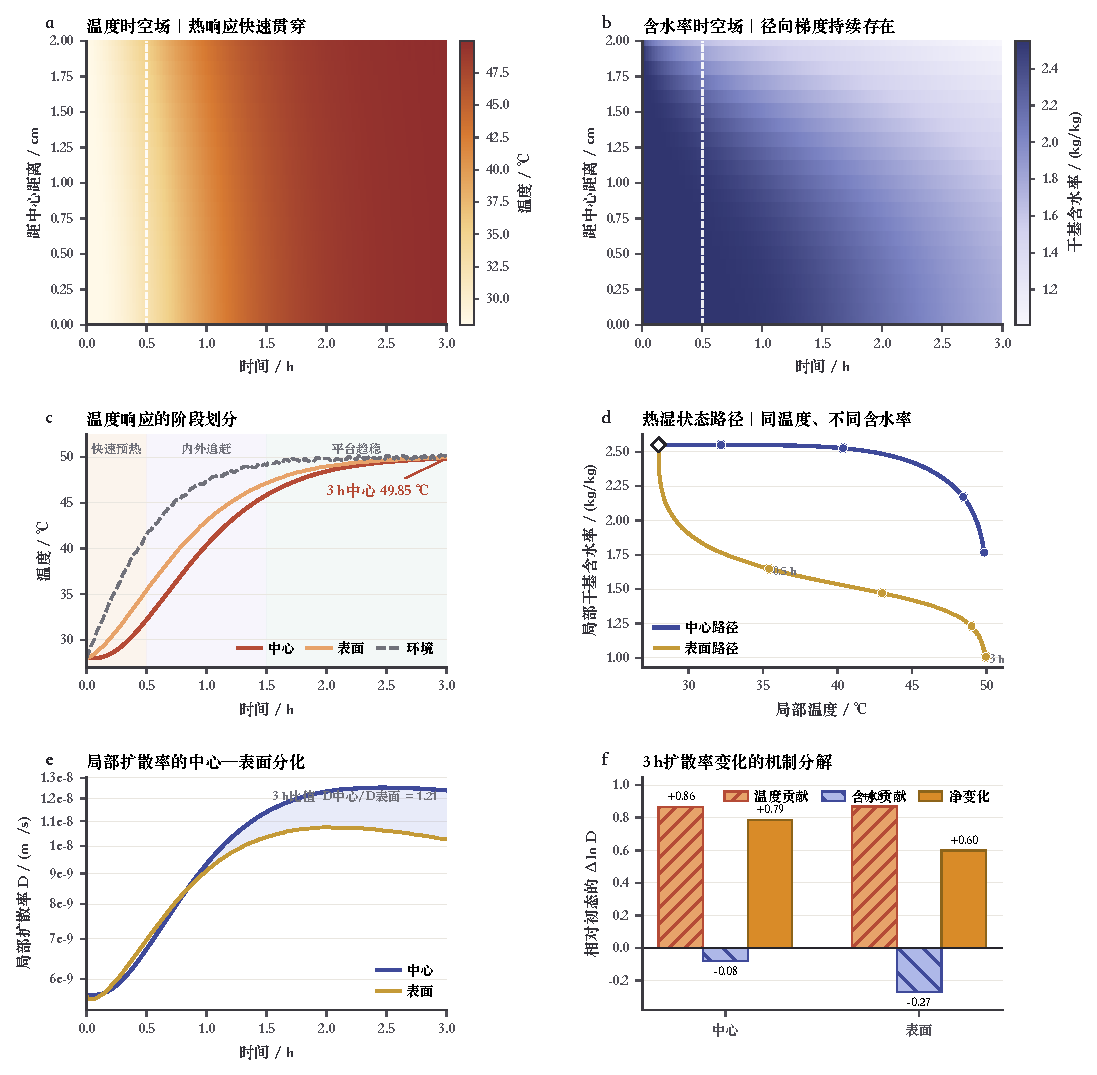
\includegraphics[width=\textwidth]{figures/fig03_q2_coupling.pdf}
  \caption{问题二耦合响应}
  \label{fig:q2-coupling}
\end{figure}

将式\eqref{eq:D-decomposition}代入3 h状态，中心的温度贡献为$+0.8648$，含水率贡献为$-0.0783$；表面分别为$+0.8691$和$-0.2699$。此时升温促进仍占上风，但表面脱水抑制更强。若只冻结$D$中的温度因子而仍求解温场，3 h中心含水率会由$1.7662$增至$2.1933$，表明忽略升温对扩散的作用会明显低估前三小时失水。该对照是模型内机制消融，不是实验因果识别。

图\ref{fig:q2-coupling}(d)把中心和表面的$(T,C)$状态路径直接投影到同一平面，可见二者在接近相同温度后仍保持不同含水率；(e)进一步显示中心扩散率与表面扩散率的分化；(f)则将$\Delta\ln D$拆成温度项、含水项和净变化。这三个面板把“场的差异”与“物性公式中的竞争机制”连接起来，而不是只给出两张结果热图。

进一步比较剖面可见，温度的中心---表面差已由早期的数摄氏度收缩到$0.1169\ ^\circ\mathrm C$，含水率差却仍为$0.7581$。这是因为热扩散时间以分钟计，而水分扩散时间以小时计；同时表层含水率下降又使其局部$D$减小，延缓内部水分向表面的补给。故“温场近似均匀”和“水分场近似均匀”在本问题中属于两个完全不同的阶段。

\subsection{问题三：全域阈值事件}

\subsubsection{事件定义与严格不等式}

问题三与问题二使用同一物性、同一初态和同一物理时钟。为避免只检查少数表格位置，定义
\begin{equation}
g(t)=\max_{0\le r\le R_0}C(r,t)-0.15,
\qquad
t_*=\inf\{t:g(t)\le 0\}.
\label{eq:event}
\end{equation}
最大值搜索包含中心、全部控制体、真实表面以及空间重建。另构造中心含水率约$0.10$、内部$r\approx1.1$ cm处峰值约$0.298$的反例，中心判据会误报达标，而式\eqref{eq:event}可正确拒绝。因此，即使本次实际轨迹的最湿点最终位于中心，也不将“中心恒为最湿”预设到算法中。

连续模型在$t_*$满足等号，严格条件$C_{\max}<0.15$通常在$t_*$后的开区间成立，不存在被取到的“最早严格时刻”。因此本文同时报告等号临界时刻和向上取整后重新核验的整数秒。

\subsubsection{全域搜索与事件定位算法}

有限体积状态位于单元中心，还需把中心轴和真实表面纳入最大值搜索。中心偶对称条件给出局部形式$C(r)=a+br^2$，由前两个单元中心值可恢复轴心值
\begin{equation}
C(0,t)=\frac{r_2^2C_1-r_1^2C_2}{r_2^2-r_1^2}.
\label{eq:axis-reconstruct}
\end{equation}
内部区间采用保形三次重建，其区间值不超过相邻节点包络；第一半单元的偶二次式关于$r^2$单调。因此事件函数只需在
\begin{equation}
\mathcal S(t)=\{C(0,t),C_1(t),\ldots,C_N(t),C_s(t)\}
\end{equation}
上取最大值，即可覆盖重建后的完整径向域，而不是只检查题目表格中的21个位置。

事件定位按以下流程执行：首先读取问题二3 h时的未舍入状态，并验证此时$g(t)>0$；随后以30 s为最大内部步长分段续算，在每个BDF片段上调用稠密输出计算$g(t)$；当检测到负方向过零时，由连续插值自动细化根的位置；最后分别回代$t_*-1$ s、$t_*$和$t_*+1$ s，并从$t_*$独立推进到下一整数秒。程序还在所有接受步与步中点检查$C_{\max}(t)$的单调性，避免由于状态重建或求根切换产生伪事件。

\subsubsection{终点与后期机制}

求得
\begin{equation}
t_*=206906.491182\ \mathrm{s}=57.4740253\ \mathrm{h},
\end{equation}
按题定格式为$57.4740$ h；首个经核验严格达标的整数秒为$206907$ s，即57 h 28 min 27 s。题定含水率结果见表\ref{tab:q3_moisture}。

\input{tables/q3_tables}

图\ref{fig:q3-endpoint}显示，终点中心值为$0.1500$，表面值已降至$0.0526$，加权平均含水率为$0.1243$。临界前后1 s的$g(t)$分别约为$+2.913\times10^{-7}$和$-2.913\times10^{-7}$，证明事件发生的是向下穿越而非采样偶然命中。

\begin{figure}[htbp]
  \centering
  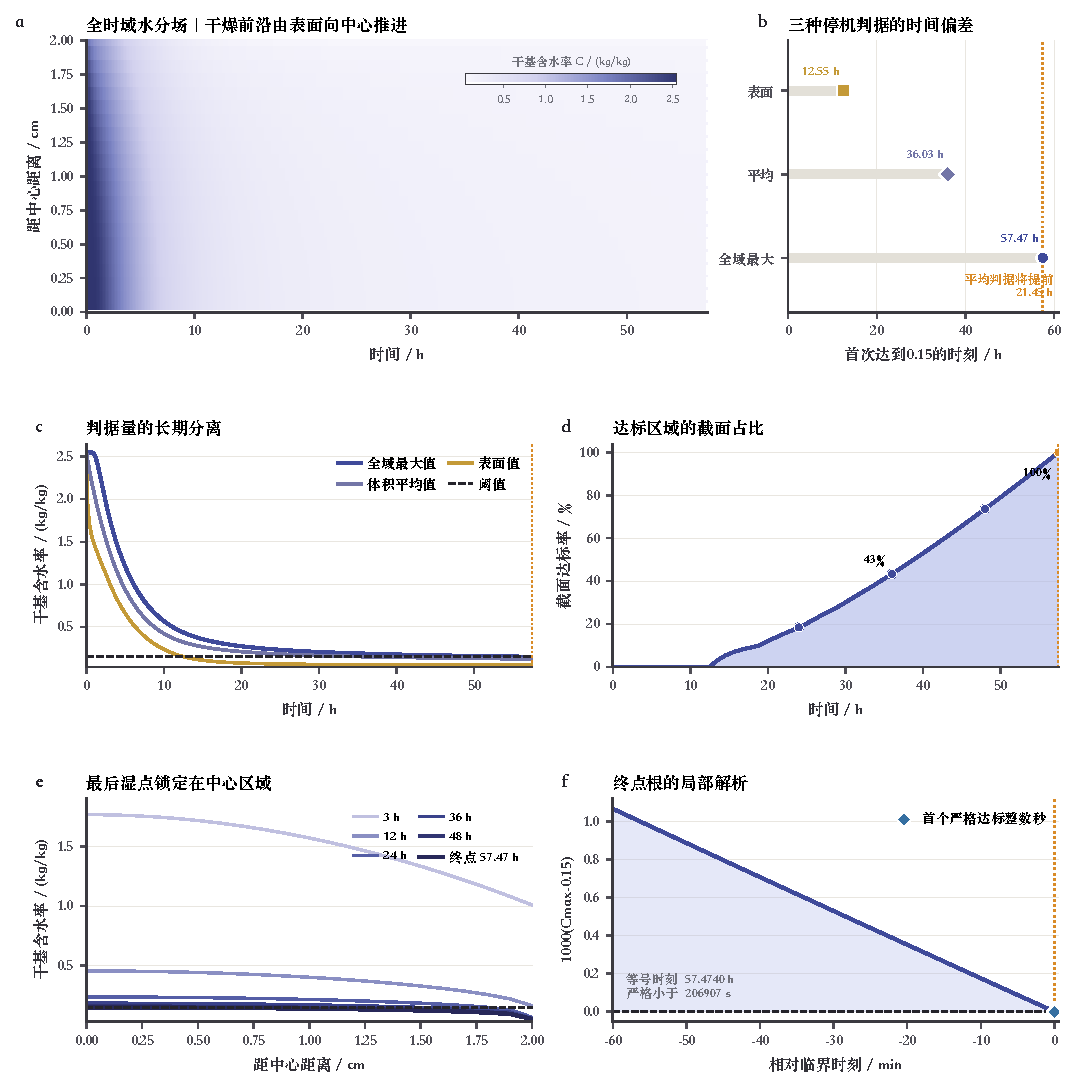
\includegraphics[width=\textwidth]{figures/fig04_q3_endpoint.pdf}
  \caption{问题三全域干燥终点}
  \label{fig:q3-endpoint}
\end{figure}

图\ref{fig:q3-endpoint}(b)量化了判据选择造成的偏差：表面值和体积平均值分别约在12.55 h和36.03 h达到$0.15$，比全域判据提前44.92 h和21.45 h；(d)显示截面达标比例虽不断增大，但必须到最后湿点达标时才达到$100\%$。在临界点，升温对$\ln D$的累计贡献约为$+0.8703$，含水率下降的贡献在中心和表面分别约为$-2.8235$和$-8.3710$。中心扩散率约$8.00\times10^{-10}\ \mathrm{m^2/s}$，表面仅约$3.12\times10^{-12}\ \mathrm{m^2/s}$，相差约257倍。低含水表层的扩散率下降与显著内部梯度共同解释了后期减速；但外部传质系数仍影响终点，故不将全过程概括为“完全由内部扩散控制”。

按全域判据，终点由最后一个达到阈值的位置控制。虽然本次主轨迹的最大值在后期位于中心，但这是求解结果而非先验条件。终点平均含水率$0.1243$明显低于阈值，表面更低至$0.0526$；若用平均值代替最大值，必然会提前停机。反之，用题定四位小数直接搜索也会把舍入误差带入事件时间，因此本文始终在未舍入状态上定位事件，只在最终表格中按格式舍入。

\subsubsection{第三问交叉验证}

为避免同一离散框架内部自洽被误认为交叉验证，另以不同空间离散、不同时间推进和独立程序复算临界事件，结果见表\ref{tab:q3-cross-validation}。其中独立程序采用P1有限元弱式、一致质量矩阵、自编BDF2与Picard迭代，并从独立求得的问题二节点末态继续；它不调用主程序的有限体积面通量、Jacobian、表面重建或事件函数。

\begin{table}[htbp]
  \caption{问题三临界时间交叉验证}
  \label{tab:q3-cross-validation}
  \centering
  \small
  \begin{tabular}{llrr}
    \toprule
    证据 & 空间与时间离散 & $t_*/\mathrm{s}$ & 相对主解$/\mathrm{s}$ \\
    \midrule
    主解 & FVM $N=1280$，BDF 30 s & 206906.491182 & --- \\
    全新复算 & 同主解，新缓存重新积分 & 206906.491182 & $0$ \\
    积分器替换 & FVM $N=1280$，Radau 30 s & 206906.491402 & $+0.000220$ \\
    空间加密 & FVM $N=2560$，BDF 30 s & 206906.415227 & $-0.075956$ \\
    独立程序 & P1 FEM $N=2560$，BDF2 3.75 s & 206906.493281 & $+0.002099$ \\
    \bottomrule
  \end{tabular}
\end{table}


五种计算的小时值均舍入为$57.4740$ h。主解网格由1280加密到2560时，临界时间改变$-0.075956$ s；按近二阶收敛估计，主网格终点的保守数值尺度约为$0.1$ s。独立有限元与主解相差$0.002099$ s，公共保存时刻的最大温差和含水率差分别为$3.028\times10^{-5}\ ^\circ\mathrm C$与$3.308\times10^{-7}$，说明不同离散路线得到一致结果，但这一毫秒级差值不作为误差上界。事件邻域回代给出
\[
g(t_*-1\ \mathrm{s})=2.913\times10^{-7},\quad
g(t_*)=0,\quad
g(206907\ \mathrm{s})=-1.482\times10^{-7},
\]
且所有接受步与步中点上的$C_{\max}$均未出现回升。水分累计守恒相对残差为$6.49\times10^{-10}$。综合网格、积分器和独立离散结果，第三问在题定四位小数下稳定；实际工艺精度仍取决于物性和边界参数。

\subsection{问题四：收缩域材料坐标模型}

\subsubsection{由干固体守恒得到移动域方程}

设$s$为单位当前体积内的干固体质量，$v$为材料速度，相对干固体的水分通量为$J_w=-sD\nabla C$。干固体与水分守恒分别为
\begin{equation}
\frac{\partial s}{\partial t}+\nabla\cdot(sv)=0,
\qquad
\frac{\partial(sC)}{\partial t}+\nabla\cdot(sCv+J_w)=0.
\end{equation}
第二式减去$C$乘第一式，得
\begin{equation}
s\frac{\mathrm DC}{\mathrm Dt}=-\nabla\cdot J_w,
\qquad
\frac{\mathrm D}{\mathrm Dt}=\frac{\partial}{\partial t}+v\cdot\nabla.
\label{eq:material-moist}
\end{equation}
仿射径向收缩且长度不变时，$v_r=(\dot R/R)r$，故
\begin{equation}
\nabla\cdot v=\frac{1}{r}\frac{\partial(rv_r)}{\partial r}
=2\frac{\dot R}{R},\qquad
\frac{\mathrm Ds}{\mathrm Dt}=-s\nabla\cdot v.
\end{equation}
若初始干固体密度$s_0$空间均匀，则
\begin{equation}
s(t)=s_0\left(\frac{R_0}{R(t)}\right)^2.
\label{eq:dry-solid-density}
\end{equation}
同一时刻的$s$与$r$无关，因而$J_w=-sD\nabla C$中的$s$可从空间散度中提出，并与式\eqref{eq:material-moist}左端约去。这是参考域水分方程不含额外$\nabla s$项的条件。

令$\xi=r/R(t)$，$u(\xi,t)=C(R(t)\xi,t)$，$\theta(\xi,t)=T(R(t)\xi,t)$。径向仿射收缩使$v=(\dot R/R)r$，网格速度$w=\dot R\xi$与材料速度一致，故材料导数在固定$\xi$处就是$u_t$。这一点可由链式法则写为
\begin{equation}
\left.\frac{\partial u}{\partial t}\right|_{\xi}
=\frac{\partial C}{\partial t}+\dot R\xi\frac{\partial C}{\partial r}
=\frac{\mathrm DC}{\mathrm Dt},
\qquad
\frac{\partial C}{\partial r}=\frac{1}{R}\frac{\partial u}{\partial\xi}.
\label{eq:ale-chain-rule}
\end{equation}
式\eqref{eq:ale-chain-rule}表明，Euler坐标中的对流项并未被忽略，而是由于网格跟随材料运动而包含在固定$\xi$的时间导数中。再将$r=R\xi$代入径向散度算子，得到参考域方程
\begin{equation}
\frac{\partial u}{\partial t}
=\frac{1}{R(t)^2\xi}\frac{\partial}{\partial\xi}
\left(\xi D(u,\theta)\frac{\partial u}{\partial\xi}\right),
\label{eq:q4-moist}
\end{equation}
\begin{equation}
b(u)\frac{\partial\theta}{\partial t}
=\frac{1}{R(t)^2\xi}\frac{\partial}{\partial\xi}
\left(\xi k(u)\frac{\partial\theta}{\partial\xi}\right).
\label{eq:q4-heat}
\end{equation}
这与移动网格/ALE思想相符\cite{kjellgren1998}。式\eqref{eq:q4-moist}依赖材料运动$v=w$、长度不变和初始$s_0$空间均匀；干基含水率的压缩效应已由干固体连续方程处理。式\eqref{eq:q4-heat}则是同一材料运动下采用的有效显热闭合，并非由干固体守恒自动推出的完整能量方程。

若误把$C$当作单位当前体积的含水量，坐标变换后会出现额外稀释或浓缩项，并导致“关闭扩散和传质后$C$仍随收缩变化”的非物理解。本文以这一极端情景作为程序单元测试：当$D=h_m=0$时，任意非均匀干基含水率剖面在材料坐标中均保持不变，从计算层面验证了式\eqref{eq:q4-moist}的守恒口径。

表面条件变为
\begin{equation}
-\frac{k}{R}\theta_\xi(1,t)=h(\theta_s-T_{\mathrm{air}}),
\qquad
-\frac{D}{R}u_\xi(1,t)=h_m(u_s-C_{\mathrm{eq}}).
\label{eq:q4-bc}
\end{equation}
按参考干质量测度，平均含水率及其累计守恒式为
\begin{equation}
\bar C(t)=2\int_0^1\xi u(\xi,t)\,\mathrm d\xi,
\end{equation}
\begin{equation}
E_C(t)=\bar C(t)-C_0+
\int_0^t\frac{2h_m}{R(\tau)}[u_s(\tau)-C_{\mathrm{eq}}(\tau)]\,\mathrm d\tau=0.
\label{eq:q4-balance}
\end{equation}

问题四物性为
\begin{align}
\hat\rho(u)&=760+90u,\\
c_p(u)&=1850+2150\frac{u}{1+u},\\
k(u)&=0.12+0.20\frac{u}{1+u},
\end{align}
\begin{equation}
D(u,\theta)=4.2\times10^{-4}
\exp\left(-\frac{0.30}{u}\right)
\exp\left[-\frac{3850}{\theta+273.15}\right].
\label{eq:q4-D}
\end{equation}

\subsubsection{参考域离散与半径驱动}

在参考网格中仍使用第\ref{eq:fvm-semidiscrete}式的环形有限体积结构。令$s_R(t)=R(t)/R_0$，则内部扩散算子整体乘以$s_R^{-2}$，而写回参考坐标的Robin系数变为$s_Rh$和$s_Rh_m$。这样可复用固定域通量程序，同时严格对应物理表面的$h,h_m$，并避免在代码中显式计算噪声较大的$\dot R(t)$。

附件半径在0--72 h内分段线性插值。每到半径观测折点，求解器与环境折点一样分段重启；若积分要求超过72 h则主动报错，防止无标记外推。每个60 s输出时刻，先在材料坐标中重建$u(\xi,t)$，再用$r=R(t)\xi$映射到物理坐标。固定物理位置$r_j$只有在$r_j\le R(t)$时才有材料场值，否则保持空白。这一规则同时用于工作簿和图\ref{fig:q4-shrinkage}的白色域外遮罩。

\subsubsection{收缩域结果}

问题四从原始初态独立计算，所得临界时刻为
\begin{equation}
t_*=183931.288720\ \mathrm{s}=51.0920246\ \mathrm{h},
\end{equation}
按题定格式为$51.0920$ h；此时$R=1.2000$ cm，首个严格达标整数秒为$183932$ s。题定输出见表\ref{tab:q4_moisture}。当固定物理位置已位于收缩后的药材外部时，表中留空；空白不表示含水率为零，动态“药材表面”列始终对应$r=R(t)$。

\input{tables/q4_tables}

图\ref{fig:q4-shrinkage}中白色区域同样表示域外。终点中心、表面和干质量加权平均含水率分别为$0.1500$、$0.0526$和$0.1184$。几何因子$1/R^2$随半径减小而增大，且面积体积比$2/R$增大；当$R/R_0=0.6$时，两者分别相对初始放大2.7778倍和1.6667倍。不过，实际扩散率同时随状态变化，故这些倍率不能直接解释成同倍数的干燥速率。

\begin{figure}[htbp]
  \centering
  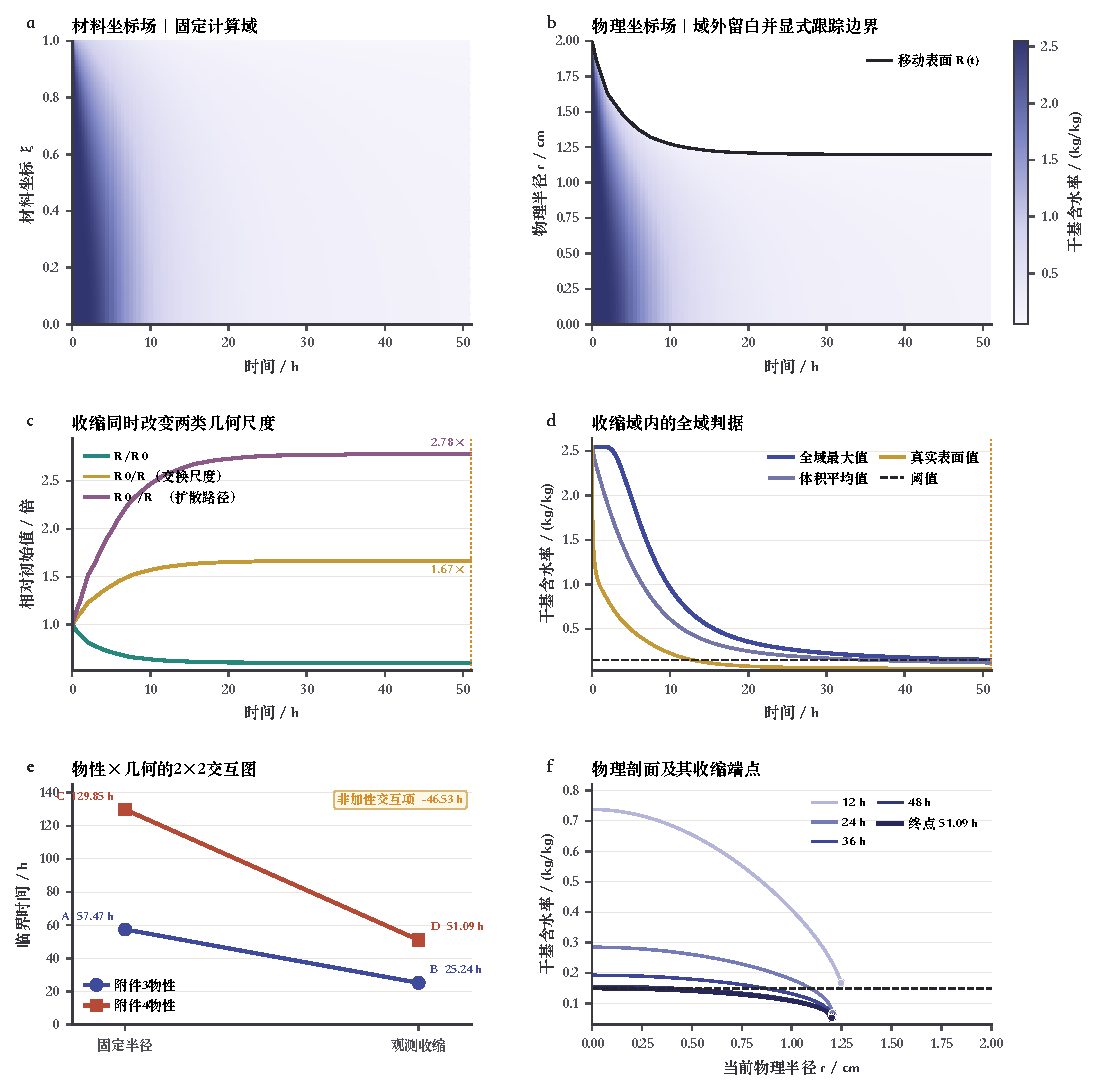
\includegraphics[width=\textwidth]{figures/fig05_q4_shrinkage.pdf}
  \caption{问题四收缩域效应}
  \label{fig:q4-shrinkage}
\end{figure}

图\ref{fig:q4-shrinkage}(a)(b)分别在材料坐标和物理坐标中呈现同一水分场，后者以移动边界和白色遮罩区分药材内外；(c)同步给出$R/R_0$、$R_0/R$与$R_0^2/R^2$，分别对应交换尺度和扩散路径尺度；(e)以四组条件情景显示几何影响随物性背景改变。

\subsubsection{统一半径轨迹下的条件对照}

问题三和问题四同时改变了几何和物性。为辨别两类改变的条件影响，令A为附录三物性与固定半径，B为附录三物性与实测收缩，C为附录四物性与固定半径，D为附录四物性与实测收缩，四组均从相同初态计算，结果见表\ref{tab:q4-factorial}。B、D使用同一条附件半径轨迹，因此这里比较的是给定外生几何驱动下的数值对照。

\begin{table}[htbp]
  \caption{几何与物性对照}
  \label{tab:q4-factorial}
  \centering
  \begin{tabular}{cllrr}
    \toprule
    场景 & 物性 & 几何 & 临界时间/h & 终点半径/cm \\
    \midrule
    A & 附录三 & 固定 & 57.4740 & 2.000 \\
    B & 附录三 & 收缩 & 25.2440 & 1.203 \\
    C & 附录四 & 固定 & 129.8484 & 2.000 \\
    D & 附录四 & 收缩 & 51.0920 & 1.200 \\
    \bottomrule
  \end{tabular}
\end{table}

以A为参考，几何与物性的简单效应及交互对比分别为
\begin{align}
\Delta_{\mathrm{geom}|\mathrm{III}}&=t_B-t_A=-32.2301\ \mathrm h,\\
\Delta_{\mathrm{prop}|\mathrm{fixed}}&=t_C-t_A=+72.3744\ \mathrm h,\\
\Delta_{\mathrm{int}}&=t_D-t_B-t_C+t_A=-46.5263\ \mathrm h.
\end{align}
三项之和为$t_D-t_A=-6.3820$ h。几何的另一简单效应为$t_D-t_C=-78.7564$ h，物性的另一简单效应为$t_D-t_B=+25.8481$ h。几何和物性的影响均随另一因素的背景而改变，$-46.5263$ h正是两组简单效应之差。

附件半径是题给输入，并未随情景物性重新求解，所以该对照描述当前模型中的条件差异。问题三、四的$6.3820$ h净差同时含有物性、几何及二者交互，并非单独的收缩贡献。

还需指出，若把问题四的经验密度同时严格解释为湿药材总密度，并要求长度固定、干固体质量守恒，则可推出$R\ge1.2112$ cm；附件半径后期低于该值。本文因此采用“有效热学系数+独立干质量守恒”的解释，而不声称同时满足严格混合物密度关系。
